\documentclass[11pt]{article}
\usepackage{amsmath, amssymb, amsthm, geometry, tikz, mathrsfs, mathtools}
\usetikzlibrary{arrows.meta, positioning, shapes, backgrounds}
\geometry{letterpaper, margin=1in}

\title{\textbf{Homework 3.3 \& 3.4 - Contrapositive and Cases: Direct Proof and Proof by Contrapositive}}
\author{Tashfeen Omran}
\date{September 2026}

\renewcommand{\qedsymbol}{$\blacksquare$}
\newtheorem{theorem}{Theorem}[section]
\newtheorem{lemma}[theorem]{Lemma}
\newtheorem{definition}[theorem]{Definition}
\newtheorem{proposition}[theorem]{Proposition}
\newtheorem{axiom}[theorem]{Axiom}

\begin{document}
\maketitle
\tableofcontents
\newpage

\section{Part 1: Comprehensive Introduction, Context, and Prerequisites}

\subsection{Historical Context and Motivation}
The foundations of rigorous mathematical proof were laid in ancient Greece, most notably by Euclid and Aristotle, who formalized deductive reasoning and propositional logic. In the late 19th and early 20th centuries, a foundational crisis in mathematics (spearheaded by paradoxes in Cantor's naive set theory) forced mathematicians like Gottlob Frege, Bertrand Russell, and David Hilbert to rigorously formalize logic. The formalized axiom systems demanded strictly defined methods of deductive verification. While direct proofs construct a clear logical chain from hypothesis $P$ to conclusion $Q$, many properties of sets and integers resist straightforward manipulation. This led to the formalization of alternative deductive routes relying on the Law of the Excluded Middle and the Law of Non-Contradiction: namely, \textbf{Proof by Contrapositive} and \textbf{Proof by Cases}. These abstract logical manipulations are not mere academic exercises; they form the very bedrock of deterministic algorithm design, probabilistic bounds, and rigorous software verification in modern Computer Science and Artificial Intelligence.

\subsection{Core Concepts \& Axioms}
At the core of this chapter are mathematical implications mapping subsets of a domain $S$. 
\begin{itemize}
    \item \textbf{Axiom of Excluded Middle:} For any proposition $P$, the statement $P \lor \neg P$ is strictly true. There is no intermediate truth value.
    \item \textbf{Logical Equivalence of Contrapositive:} In an axiomatic Boolean algebra, the implication $P \implies Q$ is logically equivalent to its contrapositive $\neg Q \implies \neg P$. This follows from the truth definition of implication: $P \implies Q \equiv \neg P \lor Q$. Reversing and negating yields $\neg(\neg Q) \lor \neg P \equiv Q \lor \neg P \equiv \neg Q \implies \neg P$.
    \item \textbf{Partitioning (Proof by Cases):} A set $S$ is partitioned by subsets $A_1, A_2, \dots, A_n$ if $\bigcup_{i=1}^n A_i = S$ and $A_i \cap A_j = \emptyset$ for all $i \neq j$. To prove $\forall x \in S, P(x)$, it is logically sufficient to prove the statement over each disjoint subset (case) $A_i$.
\end{itemize}

\subsection{Intuition and Set-Theoretic Foundations}
Think of the domain $S$ as a universe of elements. The predicate $P(x)$ acts as an indicator function (or filter) defining a subset $A \subseteq S$ where $P(x)$ is true. The predicate $Q(x)$ defines a subset $B \subseteq S$. The implication $P(x) \implies Q(x)$ is the set-theoretic claim that $A \subseteq B$. 
If verifying $x \in A \implies x \in B$ directly is algebraically difficult, we can instead look at the complements: $B^c$ and $A^c$. The statement $A \subseteq B$ is geometrically and topologically equivalent to $B^c \subseteq A^c$. This is the intuition behind the contrapositive: we assume $x \in B^c$ (i.e., $\neg Q(x)$) and prove $x \in A^c$ (i.e., $\neg P(x)$). 

\subsection{Key Theorems and Definitions}
\begin{definition}[Parity]
An integer $n \in \mathbb{Z}$ is \textbf{even} if there exists $k \in \mathbb{Z}$ such that $n = 2k$. An integer $n \in \mathbb{Z}$ is \textbf{odd} if there exists $k \in \mathbb{Z}$ such that $n = 2k + 1$. By the division algorithm, the sets of even and odd integers form a partition of $\mathbb{Z}$.
\end{definition}
\begin{theorem}[Contrapositive Equivalence]
$(P \implies Q) \iff (\sim Q \implies \sim P)$.
\end{theorem}

\subsection{Prerequisites}
To fully master this section, one must possess:
\begin{enumerate}
    \item Fluency in basic algebra over $\mathbb{Z}, \mathbb{Q}, \mathbb{R}$.
    \item Understanding of basic set operations (Union $\cup$, Intersection $\cap$, Complement $A^c$).
    \item De Morgan's Laws: $\sim(P \land Q) \equiv \sim P \lor \sim Q$ and $\sim(P \lor Q) \equiv \sim P \land \sim Q$.
    \item The ability to manipulate logical quantifiers ($\forall, \exists$).
\end{enumerate}

\newpage
\section{Part 2: Detailed Homework Solutions (Sections 3.3 \& 3.4)}

\subsection{Section 3.3 Exercises: Proof by Contrapositive}

\textbf{3.16.} Let $x \in \mathbb{Z}$. Prove that if $7x + 5$ is odd, then $x$ is even.
\begin{proof}
We use a proof by contrapositive. The contrapositive statement is: ``If $x$ is odd, then $7x+5$ is even.'' Assume $x$ is odd. By definition, there exists an integer $k$ such that $x = 2k + 1$. Substituting this into our expression yields:
\begin{align*}
    7x + 5 &= 7(2k + 1) + 5 \\
           &= 14k + 7 + 5 \\
           &= 14k + 12 \\
           &= 2(7k + 6)
\end{align*}
Since $k \in \mathbb{Z}$, closure under addition and multiplication implies $(7k + 6) \in \mathbb{Z}$. Thus, by definition, $7x + 5$ is even. Since the contrapositive is true, the original implication is true.
\end{proof}

\textbf{3.17.} Let $n \in \mathbb{Z}$. Prove that if $15n$ is even, then $9n$ is even.
\begin{proof}
We use a proof by contrapositive: ``If $9n$ is odd, then $15n$ is odd.'' Assume $9n$ is odd. The product of two integers is odd if and only if both integers are odd. Since $9$ is odd, $n$ must necessarily be odd. Let $n = 2k + 1$ for some $k \in \mathbb{Z}$. We evaluate $15n$:
\begin{align*}
    15n &= 15(2k + 1) \\
        &= 30k + 15 \\
        &= 2(15k + 7) + 1
\end{align*}
Since $(15k + 7) \in \mathbb{Z}$, $15n$ is odd. The contrapositive is proven.
\end{proof}

\textbf{3.18.} Let $x \in \mathbb{Z}$. Prove that $5x - 11$ is even if and only if $x$ is odd.
\begin{proof}
We must prove both directions of the biconditional. \\
$(\implies)$: We prove the contrapositive: ``If $x$ is even, then $5x - 11$ is odd.'' Assume $x = 2k$ for $k \in \mathbb{Z}$. 
\[ 5x - 11 = 5(2k) - 11 = 10k - 12 + 1 = 2(5k - 6) + 1 \]
Since $5k - 6 \in \mathbb{Z}$, $5x - 11$ is odd. \\
$(\impliedby)$: Assume $x$ is odd, so $x = 2m + 1$ for $m \in \mathbb{Z}$.
\[ 5x - 11 = 5(2m + 1) - 11 = 10m + 5 - 11 = 10m - 6 = 2(5m - 3) \]
Since $5m - 3 \in \mathbb{Z}$, $5x - 11$ is even. 
\end{proof}

\textbf{3.19.} Let $x \in \mathbb{Z}$. Use a lemma to prove that if $7x + 4$ is even, then $3x - 11$ is odd.
\begin{proof}
\textbf{Lemma:} If $7x + 4$ is even, then $x$ is even.
\textit{Proof of Lemma:} We prove the contrapositive. Assume $x$ is odd, so $x = 2k + 1$. Then $7x + 4 = 7(2k + 1) + 4 = 14k + 11 = 2(7k + 5) + 1$, which is odd. \\
\textbf{Main Proof:} Assume $7x + 4$ is even. By our lemma, $x$ is even, meaning $x = 2m$ for $m \in \mathbb{Z}$. Substituting this into $3x - 11$:
\[ 3x - 11 = 3(2m) - 11 = 6m - 12 + 1 = 2(3m - 6) + 1 \]
Since $3m - 6 \in \mathbb{Z}$, $3x - 11$ is odd. 
\end{proof}

\textbf{3.20.} Let $x \in \mathbb{Z}$. Prove that $3x + 1$ is even if and only if $5x - 2$ is odd.
\begin{proof}
\textbf{Lemma 1:} $3x+1$ is even $\iff x$ is odd. (Proof: $x=2k \implies 3x+1 = 6k+1$ (odd). $x=2k+1 \implies 3x+1 = 6k+4 = 2(3k+2)$ (even)). \\
\textbf{Lemma 2:} $5x-2$ is odd $\iff x$ is odd. (Proof: $x=2k \implies 5x-2 = 10k-2 = 2(5k-1)$ (even). $x=2k+1 \implies 5x-2 = 10k+3 = 2(5k+1)+1$ (odd)). \\
Since both statements are logically equivalent to ``$x$ is odd'', they are logically equivalent to each other.
\end{proof}

\textbf{3.21.} Let $n \in \mathbb{Z}$. Prove that $(n + 1)^2 - 1$ is even if and only if $n$ is even.
\begin{proof}
Note that $(n + 1)^2 - 1 = n^2 + 2n$. \\
$(\implies)$: By contrapositive. Assume $n$ is odd, so $n = 2k + 1$. 
\[ n^2 + 2n = (2k + 1)^2 + 2(2k + 1) = 4k^2 + 4k + 1 + 4k + 2 = 2(2k^2 + 4k + 1) + 1 \]
This is odd. \\
$(\impliedby)$: Assume $n = 2k$. Then $n^2 + 2n = 4k^2 + 4k = 2(2k^2 + 2k)$, which is even.
\end{proof}

\textbf{3.22.} Let $S = \{2, 3, 4\}$ and let $n \in S$. Use a proof by contrapositive to prove that if $n^2(n - 1)^2/4$ is even, then $n^2(n + 1)^2/4$ is even.
\begin{proof}
The contrapositive statement is: ``If $\frac{n^2(n + 1)^2}{4}$ is odd, then $\frac{n^2(n - 1)^2}{4}$ is odd, for $n \in S$.'' We test all $n \in S$:
\begin{itemize}
    \item $n = 2$: $\frac{2^2(3)^2}{4} = 9$ (odd). The premise is true. We check the conclusion: $\frac{2^2(1)^2}{4} = 1$ (odd). True.
    \item $n = 3$: $\frac{3^2(4)^2}{4} = 36$ (even). Premise is false, implication is vacuously true.
    \item $n = 4$: $\frac{4^2(5)^2}{4} = 100$ (even). Premise is false, implication is vacuously true.
\end{itemize}
Since the contrapositive holds for all $n \in S$, the original implication is true.
\end{proof}

\textbf{3.23.} Let $A = \{0, 1, 2\}$ and $B = \{4, 5, 6\}$ be subsets of $S = \{0, 1, \dots, 6\}$. Let $n \in S$. Prove that if $\frac{n(n - 1)(n - 2)}{6}$ is even, then $n \in A \cup B$.
\begin{proof}
By contrapositive: ``If $n \notin A \cup B$, then $\frac{n(n - 1)(n - 2)}{6}$ is odd.'' \\
Since $S = \{0, 1, 2, 3, 4, 5, 6\}$ and $A \cup B = \{0, 1, 2, 4, 5, 6\}$, the only element in $S$ not in $A \cup B$ is $3$. Thus, we assume $n = 3$. We evaluate the expression:
\[ \frac{3(3 - 1)(3 - 2)}{6} = \frac{3(2)(1)}{6} = \frac{6}{6} = 1 \]
Since $1$ is an odd integer, the contrapositive is proven.
\end{proof}

\textbf{3.24.} Let $n \in \mathbb{Z}$. Prove that $2n^2 + n$ is odd if and only if $\cos\left(\frac{n\pi}{2}\right)$ is even.
\begin{proof}
First, $\cos(\frac{n\pi}{2})$ evaluates to $0$ if $n$ is odd, and $\pm 1$ if $n$ is even. In the integers, $0$ is even ($0 = 2(0)$) and $\pm 1$ are odd. Thus, $\cos(\frac{n\pi}{2})$ is even $\iff n$ is odd. We must therefore prove $2n^2 + n$ is odd $\iff n$ is odd. \\
$(\implies)$: By contrapositive. Assume $n$ is even ($n = 2k$). $2(2k)^2 + 2k = 8k^2 + 2k = 2(4k^2 + k)$, which is even. \\
$(\impliedby)$: Assume $n$ is odd ($n = 2k + 1$). $2(2k + 1)^2 + (2k + 1) = 2(4k^2 + 4k + 1) + 2k + 1 = 8k^2 + 10k + 3 = 2(4k^2 + 5k + 1) + 1$, which is odd. 
\end{proof}

\textbf{3.25.} Let $\{A, B\}$ be a partition of $S = \{1, 2, \dots, 7\}$, where $A = \{1, 4, 5\}$ and $B = \{2, 3, 6, 7\}$. Prove that if $\frac{n^2 + 3n - 4}{2}$ is even, then $n \in A$.
\begin{proof}
By contrapositive: ``If $n \notin A$, then $\frac{n^2 + 3n - 4}{2}$ is odd.'' Since $A$ and $B$ partition $S$, $n \notin A \implies n \in B$. We evaluate the expression for all $n \in \{2, 3, 6, 7\}$:
\begin{itemize}
    \item $n=2: \frac{4 + 6 - 4}{2} = 3$ (odd).
    \item $n=3: \frac{9 + 9 - 4}{2} = 7$ (odd).
    \item $n=6: \frac{36 + 18 - 4}{2} = 25$ (odd).
    \item $n=7: \frac{49 + 21 - 4}{2} = 33$ (odd).
\end{itemize}
The expression is odd in all cases, verifying the contrapositive.
\end{proof}

\subsection{Section 3.4 Exercises: Proof by Cases}

\textbf{3.26.} Prove that if $n \in \mathbb{Z}$, then $n^2 - 3n + 9$ is odd.
\begin{proof}
We proceed by cases on the parity of $n$. \\
\textbf{Case 1:} $n$ is even ($n = 2k$). 
\[ n^2 - 3n + 9 = (2k)^2 - 3(2k) + 9 = 4k^2 - 6k + 9 = 2(2k^2 - 3k + 4) + 1 \]
Since $(2k^2 - 3k + 4) \in \mathbb{Z}$, the result is odd. \\
\textbf{Case 2:} $n$ is odd ($n = 2k + 1$).
\[ (2k + 1)^2 - 3(2k + 1) + 9 = 4k^2 + 4k + 1 - 6k - 3 + 9 = 4k^2 - 2k + 7 = 2(2k^2 - k + 3) + 1 \]
Since $(2k^2 - k + 3) \in \mathbb{Z}$, the result is odd. Both mutually exhaustive cases yield an odd integer.
\end{proof}

\textbf{3.27.} Prove that if $n \in \mathbb{Z}$, then $n^3 - n$ is even.
\begin{proof}
We factor $n^3 - n = n(n^2 - 1) = (n-1)n(n+1)$. We proceed by cases. \\
\textbf{Case 1:} $n$ is even ($n = 2k$). Then $n^3 - n = 2k(4k^2 - 1) = 2(4k^3 - k)$, which is even. \\
\textbf{Case 2:} $n$ is odd ($n = 2k + 1$). Then $n^3 - n = (2k + 1)((2k + 1)^2 - 1) = (2k + 1)(4k^2 + 4k) = 2[2k(k + 1)(2k + 1)]$, which is even.
\end{proof}

\textbf{3.28.} Let $x, y \in \mathbb{Z}$. Prove that if $xy$ is odd, then $x$ and $y$ are odd.
\begin{proof}
We use a proof by contrapositive: ``If $x$ is even or $y$ is even, then $xy$ is even.'' We evaluate the cases representing this logical disjunction. \\
\textbf{Case 1:} $x$ is even ($x = 2k, k \in \mathbb{Z}$). Let $y \in \mathbb{Z}$ be arbitrary. $xy = (2k)y = 2(ky)$. This is even. \\
\textbf{Case 2:} $y$ is even ($y = 2m, m \in \mathbb{Z}$). Let $x \in \mathbb{Z}$ be arbitrary. $xy = x(2m) = 2(xm)$. This is even. \\
Because $xy$ is even in all exhaustive cases of the contrapositive premise, the theorem holds.
\end{proof}

\textbf{3.29.} Let $a, b \in \mathbb{Z}$. Prove that if $ab$ is odd, then $a^2 + b^2$ is even.
\begin{proof}
If $ab$ is odd, then by the result of Problem 3.28, both $a$ and $b$ must be odd. Let $a = 2k + 1$ and $b = 2m + 1$ for integers $k, m$.
\[ a^2 + b^2 = (2k + 1)^2 + (2m + 1)^2 = 4k^2 + 4k + 1 + 4m^2 + 4m + 1 = 2(2k^2 + 2k + 2m^2 + 2m + 1) \]
Since the term in parentheses is an integer, the sum is even.
\end{proof}

\textbf{3.30.} Let $x, y \in \mathbb{Z}$. Prove that $x - y$ is even if and only if $x$ and $y$ are of the same parity.
\begin{proof}
$(\implies)$: We prove the contrapositive: if $x$ and $y$ have opposite parity, then $x - y$ is odd. Without loss of generality, assume $x = 2k$ and $y = 2m + 1$. 
\[ x - y = 2k - (2m + 1) = 2k - 2m - 2 + 1 = 2(k - m - 1) + 1 \]
This is an odd integer. \\
$(\impliedby)$: Assume $x$ and $y$ have the same parity. \\
\textbf{Case 1:} Both are even ($x = 2k, y = 2m$). $x - y = 2(k - m)$, which is even. \\
\textbf{Case 2:} Both are odd ($x = 2k + 1, y = 2m + 1$). $x - y = (2k + 1) - (2m + 1) = 2(k - m)$, which is even.
\end{proof}

\textbf{3.31.} Let $a, b \in \mathbb{Z}$. Prove that if $a + b$ and $ab$ are of the same parity, then $a$ and $b$ are even.
\begin{proof}
We analyze all combinations of parity for $a$ and $b$. \\
\textbf{Case 1:} $a$ even, $b$ even. Then $a+b$ is even, $ab$ is even. (Same parity). \\
\textbf{Case 2:} $a$ odd, $b$ odd. Then $a+b$ is even, $ab$ is odd. (Different parity). \\
\textbf{Case 3:} One even, one odd. Then $a+b$ is odd, $ab$ is even. (Different parity). \\
The hypothesis strictly limits us to the domain where $a+b$ and $ab$ share parity. This only occurs in Case 1, establishing that $a$ and $b$ must be even.
\end{proof}

\textbf{3.32.} (a) Let $x$ and $y$ be integers. Prove that $(x + y)^2$ is even if and only if $x$ and $y$ are of the same parity.
\begin{proof}
$(\implies)$: Contrapositive. Assume $x,y$ are of opposite parity. Their sum $x+y$ is odd (sum of even and odd). The square of an odd integer $(x+y)^2$ is odd. \\
$(\impliedby)$: Assume $x,y$ have the same parity. Their sum $x+y$ is even (sum of two evens or two odds is even). The square of an even integer $(x+y)^2$ is even.
\end{proof}
\noindent (b) Restate the result in terms of odd integers: \textit{``Let $x$ and $y$ be integers. $(x + y)^2$ is odd if and only if $x$ and $y$ are of opposite parity.''}

\textbf{3.33.} Let $A = \{1, 2, 3\}$ and $B = \{2, 3, 4\}$ be subsets of $S = \{1, 2, 3, 4\}$. Prove that $2n^2 - 5n$ is either (a) positive and even or (b) negative and odd iff $n \notin A \cap B$.
\begin{proof}
The intersection is $A \cap B = \{2, 3\}$. The condition $n \notin A \cap B$ within $S$ is equivalent to $n \in \{1, 4\}$. \\
$(\implies)$: By contrapositive. Assume $n \in A \cap B$. 
If $n = 2$: $2(4) - 10 = -2$ (negative and even; violates both a and b).
If $n = 3$: $2(9) - 15 = 3$ (positive and odd; violates both a and b). \\
$(\impliedby)$: Assume $n \in \{1, 4\}$.
If $n = 1$: $2(1) - 5 = -3$ (negative and odd; satisfies b).
If $n = 4$: $2(16) - 20 = 12$ (positive and even; satisfies a).
\end{proof}

\textbf{3.34.} Let $A = \{3, 4\}$ be a subset of $S = \{1, 2, 3, 4, 5, 6\}$. Let $n \in S$. Prove that if $\frac{n^2(n + 1)^2}{4}$ is even, then $n \in A$.
\begin{proof}
By contrapositive. Assume $n \notin A$, meaning $n \in \{1, 2, 5, 6\}$. 
\begin{itemize}
    \item $n=1: \frac{1(4)}{4} = 1$ (odd).
    \item $n=2: \frac{4(9)}{4} = 9$ (odd).
    \item $n=5: \frac{25(36)}{4} = 225$ (odd).
    \item $n=6: \frac{36(49)}{4} = 441$ (odd).
\end{itemize}
In all exhaustive cases, the expression is odd. Thus, the implication holds.
\end{proof}

\textbf{3.35.} Prove for every nonnegative integer $n$ that $2^n + 6^n$ is an even integer.
\begin{proof}
We partition the nonnegative integers into two cases: $n = 0$ and $n \ge 1$. \\
\textbf{Case 1:} $n = 0$. $2^0 + 6^0 = 1 + 1 = 2$, which is even. \\
\textbf{Case 2:} $n \ge 1$. $2^n = 2(2^{n-1})$, which is even since $2^{n-1}$ is an integer. Similarly, $6^n = 6(6^{n-1}) = 2(3 \cdot 6^{n-1})$, which is even. The sum of two even integers is even.
\end{proof}

\textbf{3.36.} Let $x, y \in \mathbb{Z}$. Prove that if $3x + 4y$ and $4x + 5y$ are both even, then $x$ and $y$ are both even.
\begin{proof}
Assume $3x + 4y$ and $4x + 5y$ are even. The difference of two even integers is even: $(4x + 5y) - (3x + 4y) = x + y$. Thus, $x + y$ is even, which means $x$ and $y$ share the same parity. 
Suppose both are odd. Let $x = 2a + 1$ and $y = 2b + 1$. 
\[ 3x + 4y = 3(2a + 1) + 4(2b + 1) = 6a + 3 + 8b + 4 = 2(3a + 4b + 3) + 1 \]
This implies $3x + 4y$ is odd, contradicting our premise. Thus, both $x$ and $y$ must be even.
\end{proof}

\textbf{3.37.} Let $x, y, z \in \mathbb{Z}$. Prove that if exactly two of the three integers are even, then $3x + 5y + 7z$ is odd.
\begin{proof}
We proceed by analyzing the exhaustive cases for which two variables are even and one is odd. Note that the coefficients $3, 5, 7$ are all odd. \\
\textbf{Case 1:} $x$ is odd ($2a+1$), $y, z$ are even ($2b, 2c$). 
\[ 3(2a+1) + 5(2b) + 7(2c) = 6a + 3 + 10b + 14c = 2(3a + 5b + 7c + 1) + 1 \text{ (odd)} \]
\textbf{Case 2:} $y$ is odd, $x, z$ are even. The odd term is $5(2b+1) = 10b+5$. The other terms are even. The sum of an odd and two evens is odd. \\
\textbf{Case 3:} $z$ is odd, $x, y$ are even. The odd term is $7(2c+1) = 14c+7$. The sum is odd. \\
In all cases, the expression evaluates to an odd integer.
\end{proof}

\textbf{3.38.} Let $S = \{8, 12, 20, 24\}$. Prove that if $\{x, y\}$ is a 2-element subset of $S$, then either $x + y = 8k$ for some even $k$ or $x + y = 4\ell$ for some odd $\ell$.
\begin{proof}
We exhaust all 2-element subsets of $S$:
\begin{itemize}
    \item $\{8, 12\}: 8+12=20 = 4(5)$. Here $\ell=5$ (odd).
    \item $\{8, 20\}: 8+20=28 = 4(7)$. Here $\ell=7$ (odd).
    \item $\{8, 24\}: 8+24=32 = 8(4)$. Here $k=4$ (even).
    \item $\{12, 20\}: 12+20=32 = 8(4)$. Here $k=4$ (even).
    \item $\{12, 24\}: 12+24=36 = 4(9)$. Here $\ell=9$ (odd).
    \item $\{20, 24\}: 20+24=44 = 4(11)$. Here $\ell=11$ (odd).
\end{itemize}
Every pair satisfies the disjunction.
\end{proof}

\textbf{3.39.} Let $A, B$ and $C$ be sets. Prove that if $x \notin A \cup B$ and $x \notin B \cup C$, then $x \notin A \cup C$.
\begin{proof}
By the definition of the union complement (De Morgan's Laws for Sets), $x \notin A \cup B \implies x \notin A \land x \notin B$. Furthermore, $x \notin B \cup C \implies x \notin B \land x \notin C$. We deduce that $x \notin A$ and $x \notin C$. Therefore, $x \notin A \cup C$. 
\end{proof}

\textbf{3.40.} Cover vs Partition Proof Evaluation. \\
Result: Let $a, b \in \mathbb{Z}$. If $a$ is even or $b$ is even, then $ab$ is even. 
\begin{proof}
(a) Why is $\{S_1, S_2, S_3\}$ (where $S_1$ is both odd, $S_2$ is $a$ even, $S_3$ is $b$ even) a cover but not a partition of $\mathbb{Z} \times \mathbb{Z}$? \\
A partition requires mutually disjoint sets. Here, $S_2 \cap S_3 = \{(a,b) \mid a \text{ is even and } b \text{ is even}\} \neq \emptyset$. \\
(b) Why does the set $S_1$ not appear in the proof? \\
Because the implication $P \implies Q$ requires assuming the premise $P$ (``$a$ is even or $b$ is even''). The domain subset $S_1$ violates $P$. \\
(c) Give a proof by cases where cases are a partition, not a cover. \\
Let the premise hold. We partition the premise space into:
\textbf{Case 1:} $a$ is even, $b \in \mathbb{Z}$. Let $a = 2k$. Then $ab = 2(kb)$, which is even. \\
\textbf{Case 2:} $a$ is odd, $b$ is even. Let $b = 2m$. Then $ab = a(2m) = 2(am)$, which is even. \\
These two cases are disjoint and their union fully covers the condition ``$a$ is even or $b$ is even''.
\end{proof}

\newpage
\section{Part 3: In-Depth Analysis of Problems and Techniques}

\subsection{A) Problem Types and Logical Strategies}
The homework exercises fall into two rigorous logical paradigms:
\begin{enumerate}
    \item \textbf{Implication Testing via Contrapositive (e.g., 3.16 - 3.25):} Used when the conclusion of an implication is simpler to algebraically construct than its hypothesis. The strategy involves negating the target conclusion, pushing the negation through quantifiers/expressions using parity definitions, and algebraically resolving the original negated hypothesis.
    \item \textbf{Domain Exhaustion / Proof by Cases (e.g., 3.26 - 3.40):} Used when the domain is implicitly disjoint (e.g., parity divides $\mathbb{Z}$ into even and odd sets). The overarching strategy involves defining mutually exclusive and collectively exhaustive subspaces $C_i \subseteq \Omega$ such that $\bigcup C_i = \Omega$. 
\end{enumerate}

\subsection{B) Key Analytical and Logical Manipulations}
\begin{itemize}
    \item \textbf{De Morgan's Logical Trick:} In Problem 3.28 (``If $xy$ is odd, then $x$ and $y$ are odd''), manipulating the direct proof is analytically impossible without rational numbers. By utilizing the contrapositive, $\sim(x \text{ odd} \land y \text{ odd}) \equiv x \text{ even} \lor y \text{ even}$, we convert an intersection requirement into a union of manageable cases.
    \item \textbf{Factoring to Reveal Parity Sequences:} In Problem 3.27 ($n^3-n$), pulling the term into $n(n^2-1) = (n-1)n(n+1)$ reveals consecutive integers. This ensures one term is always even, a highly efficient trick for modular arithmetic logic.
    \item \textbf{Biconditional Splitting:} In problems like 3.18, 3.20, and 3.30, the $\iff$ statement was split into $(\implies)$ and $(\impliedby)$. It is analytically safer to prove one direction directly, and the converse via its contrapositive, bypassing messy inverse algebra.
\end{itemize}

\section{Part 4: Cheatsheet, Visuals, and Tips for Success}

\subsection{Theorems \& Logical Equivalences}
\begin{itemize}
    \item \textbf{Contrapositive:} $P \implies Q \equiv \sim Q \implies \sim P$
    \item \textbf{Converse (NOT strictly equivalent to implication):} $Q \implies P$
    \item \textbf{Inverse (NOT strictly equivalent to implication):} $\sim P \implies \sim Q$
    \item \textbf{De Morgan's Laws (Sets):} $(A \cup B)^c = A^c \cap B^c$ and $(A \cap B)^c = A^c \cup B^c$
\end{itemize}

\subsection{Set \& Logic Illustrations}

Below is an illustration utilizing \texttt{TikZ} to visualize how Proof by Cases partitions a logical sample space $\Omega$, establishing $Q$ across mutually exclusive domains.

\vspace{0.5cm}
\begin{center}
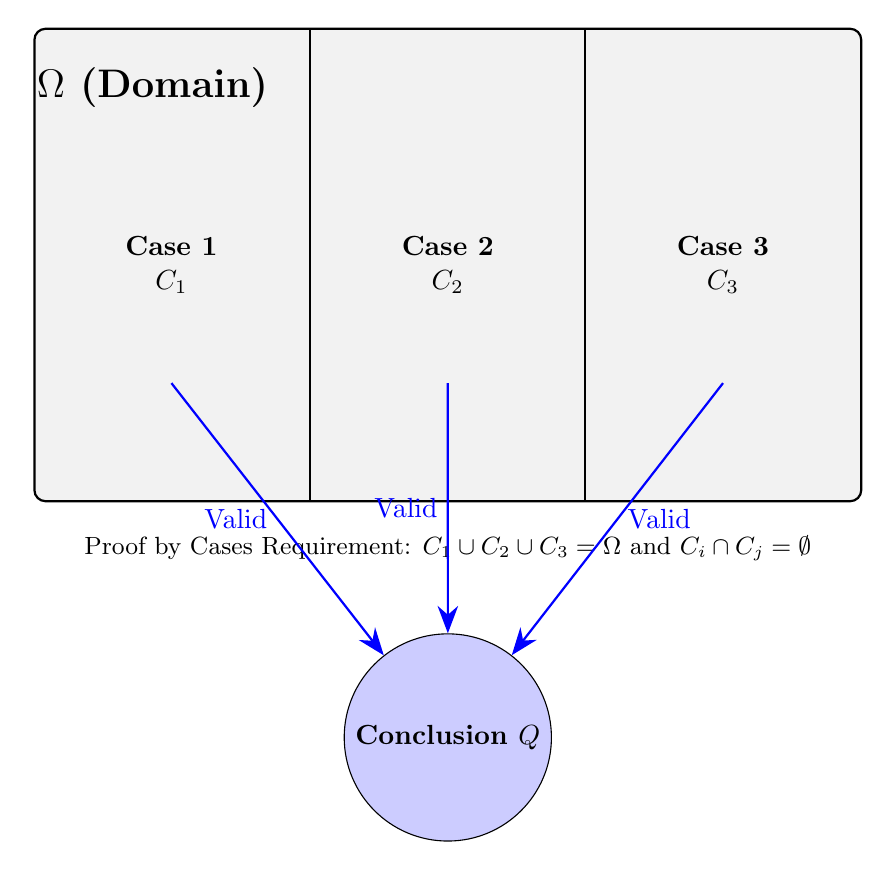
\begin{tikzpicture}[scale=1.5]
    % Outer space
    \draw[thick, rounded corners, fill=gray!10] (0,0) rectangle (7,4);
    \node[font=\bfseries\Large] at (1, 3.5) {$\Omega$ (Domain)};
    
    % Partitions
    \draw[thick] (2.33,0) -- (2.33,4);
    \draw[thick] (4.66,0) -- (4.66,4);
    
    % Nodes
    \node[font=\bfseries, text width=2cm, align=center] at (1.16, 2) {Case 1\\ $C_1$};
    \node[font=\bfseries, text width=2cm, align=center] at (3.5, 2) {Case 2\\ $C_2$};
    \node[font=\bfseries, text width=2cm, align=center] at (5.83, 2) {Case 3\\ $C_3$};
    
    % Equations
    \node[font=\small] at (3.5, -0.4) {Proof by Cases Requirement: $C_1 \cup C_2 \cup C_3 = \Omega$ and $C_i \cap C_j = \emptyset$};
    
    % Mappings to Q
    \node[circle, draw, fill=blue!20, minimum size=1cm, font=\bfseries] (Q) at (3.5, -2) {Conclusion $Q$};
    \draw[-{Stealth[scale=1.5]}, thick, blue] (1.16, 1) -- (Q) node[midway, left] {Valid};
    \draw[-{Stealth[scale=1.5]}, thick, blue] (3.5, 1) -- (Q) node[midway, left] {Valid};
    \draw[-{Stealth[scale=1.5]}, thick, blue] (5.83, 1) -- (Q) node[midway, right] {Valid};
\end{tikzpicture}
\end{center}

\subsection{Heuristics, "Cheats", and Pitfalls}
\begin{itemize}
    \item \textbf{Heuristic for Contrapositive:} Use this when the conclusion $Q$ has the word "or" ($\lor$). By negating $Q$, De Morgan's Law gives you an "and" ($\land$) in your premise, which is far easier to assume!
    \item \textbf{Fallacy - Affirming the Consequent:} Assuming $Q$ is true, and deducing $P$ is true. This proves the \textit{converse}, not the implication. 
    \item \textbf{Probability Trap - Base Rate Fallacy:} The statistical manifestation of reversing implication. Knowing $P(B|A)$ does not mean $P(A|B)$ is high. The logical contrapositive strictly corresponds to $P(A^c | B^c) = 1$ when $P(B|A) = 1$.
\end{itemize}

\newpage
\section{Part 5: Conceptual Synthesis and The "Big Picture"}

\subsection{A) Thematic Connections}
The central theme unifying this chapter is the \textbf{Isomorphism of Boolean Logic and Set Theory}. The statement $P \implies Q$ is an assertion of topological containment ($P \subseteq Q$). Proof by contrapositive operates algebraically on the complements ($Q^c \subseteq P^c$). This serves as a vital bridge to understanding sigma-algebras ($\sigma$-algebras) in measure theory, where the complement of a measurable set must strictly remain within the measurable space.

\subsection{B) Forward and Backward Links}
Backward, this chapter mechanizes basic arithmetic axioms. Forward, Proof by Cases forms the discrete analogue to \textbf{Lebesgue Integration}. When we partition a set into cases $C_i$, and verify conditions on those disjoint pieces, we are building simple functions. As cases approach infinity, discrete logical sums translate directly into measure-theoretic integrals.

\section{Part 6: Abstract Real-World Modeling (AI, ML, \& Quant Finance)}

\subsection{A) Concrete Scenarios}
\begin{enumerate}
    \item \textbf{Credit Counterparty Risk (Quant Finance):} In modeling structural default using Merton frameworks, default contagion implies: if Firm A survives ($P$), then Firm B survives ($Q$). The contrapositive dynamically forces quantitative models to recognize that Firm B defaulting ($\sim Q$) immediately guarantees Firm A defaults ($\sim P$).
    \item \textbf{Random Forest Partitioning (Machine Learning):} Decision trees utilize strict \textit{Proof by Cases}. The feature space $\mathbb{R}^n$ is recursively partitioned into mutually exclusive leaves $C_1, C_2, \dots, C_k$.
\end{enumerate}

\subsection{B) Model Problem Setup: Algorithmic Arbitrage Pricing State-Space}
Let us formalize a financial scenario utilizing the rigorous logic of \textbf{Proof by Cases} extended to Stochastic Measure Theory (The Law of Total Probability). \\
Let $(\Omega, \mathcal{F}, \mathbb{P})$ be a probability space representing all possible states of a market at time $T$. Let $X(\omega)$ be the payoff of a derivative. A quant researcher wishes to prove that the expected payoff $\mathbb{E}[X] > 0$ under a risk-neutral measure $\mathbb{Q}$.
\begin{proof}
Define a measurable partition of $\Omega$ representing market volatility regimes: $V_1$ (Contraction), $V_2$ (Normal), $V_3$ (Expansion). By definition of a partition, $\bigcup_{i=1}^3 V_i = \Omega$ and $V_i \cap V_j = \emptyset$. \\
By the Radon-Nikodym theorem and properties of conditional expectation over cases, the total expected payoff is structurally equivalent to a Proof by Cases:
\[ \mathbb{E}^{\mathbb{Q}}[X] = \int_{\Omega} X(\omega) d\mathbb{Q} = \sum_{i=1}^3 \int_{V_i} X(\omega) d\mathbb{Q} = \sum_{i=1}^3 \mathbb{E}^{\mathbb{Q}}[X \mid V_i] \mathbb{Q}(V_i) \]
To guarantee $\mathbb{E}^{\mathbb{Q}}[X] > 0$, the algorithmic logic requires verifying the condition in each case: $\mathbb{E}[X \mid V_1] > 0$, $\mathbb{E}[X \mid V_2] > 0$, and $\mathbb{E}[X \mid V_3] > 0$. If verified, the trading algorithm is mathematically guaranteed positive expectation.
\end{proof}

\newpage
\section{Part 7: Common Variations and Untested Concepts}

The standard curriculum following Sections 3.3 (Contrapositive) and 3.4 (Cases) introduces \textbf{Proof by Contradiction (Reductio ad Absurdum)}, an extension of the contrapositive logic utilizing the Axiom of Non-Contradiction.

\begin{theorem}
$\sqrt{2}$ is irrational.
\end{theorem}
\begin{proof}
Assume, for the sake of contradiction, that $\sqrt{2}$ is rational. Then it can be expressed as a fraction in lowest terms: $\sqrt{2} = \frac{a}{b}$, where $a, b \in \mathbb{Z}$, $b \neq 0$, and $\gcd(a,b) = 1$ (they share no common factors, so they cannot both be even). \\
Squaring both sides yields $2 = \frac{a^2}{b^2}$, which implies $a^2 = 2b^2$. \\
Since $b^2$ is an integer, $a^2$ is even. By a previously proven lemma (see 3.21 logical equivalent), if $a^2$ is even, then $a$ is even. Let $a = 2k$. \\
Substitute $a$ back into the equation: $(2k)^2 = 2b^2 \implies 4k^2 = 2b^2 \implies b^2 = 2k^2$. \\
This implies $b^2$ is even, which means $b$ must also be even. \\
We have deduced that both $a$ and $b$ are even, contradicting our assumption that $\gcd(a,b) = 1$. The initial assumption must be false. Therefore, $\sqrt{2}$ is irrational.
\end{proof}

\section{Part 8: Advanced Diagnostic Testing: "Find the Flaw"}

Below are 5 exceptionally convincing, yet flawed, mathematical proofs. Find the logical error in each.

\subsection{Flawed Proofs}

\textbf{Problem 1: (Contrapositive Error)}
\textit{Theorem:} Let $x, y \in \mathbb{R}$. If $x > 0$ and $y > 0$, then $xy > 0$.
\textit{Proof:} We proceed by contrapositive. Assume $xy \le 0$. By the contrapositive definition, we must show $x \le 0$ and $y \le 0$. If $xy$ is negative or zero, both numbers cannot be positive. Hence, $x \le 0$ and $y \le 0$. The proof is complete. $\blacksquare$

\textbf{Problem 2: (Case Overlap Flaw)}
\textit{Theorem:} Let $n \in \mathbb{Z}$. Then $n^2 \ge n$.
\textit{Proof:} We use Proof by Cases. \\
\textit{Case 1:} $n$ is a positive integer ($n \ge 1$). Multiplying both sides of $n \ge 1$ by the positive integer $n$ yields $n^2 \ge n$. \\
\textit{Case 2:} $n$ is a negative integer ($n \le -1$). Since $n^2 \ge 0$ and $n < 0$, by transitivity, $n^2 \ge n$. \\
Since we have checked the cases, $n^2 \ge n$ for all $n \in \mathbb{Z}$. $\blacksquare$

\textbf{Problem 3: (Vacuous Logic Error)}
\textit{Theorem:} For all $x \in \mathbb{R}$, if $x^2 + 1 < 0$, then $x = 100$.
\textit{Proof:} Since $x^2 \ge 0$ for all real numbers, $x^2 + 1 \ge 1$. Therefore, the hypothesis $x^2 + 1 < 0$ is impossible. Because the hypothesis is false, the implication implies that $x$ must indeed equal $100$ in reality. $\blacksquare$

\textbf{Problem 4: (Converse mistaken for Contrapositive)}
\textit{Theorem:} If an integer $n$ is divisible by 4, it is even.
\textit{Proof:} We proceed by assuming the conclusion. If $n$ is even, then $n = 2k$. We can rewrite this as $n = 4(\frac{k}{2})$. Thus, $n$ is divisible by 4. The implication holds. $\blacksquare$

\textbf{Problem 5: (Division by Zero in Cases)}
\textit{Theorem:} For all $x \in \mathbb{R}$, $x^2 - x = 0 \implies x = 1$.
\textit{Proof:} We proceed by evaluating the algebraic condition $x^2 - x = 0$. Factoring out $x$, we get $x(x - 1) = 0$. Dividing both sides of the equation by $x$ yields $x - 1 = 0$, which implies $x = 1$. The theorem is verified. $\blacksquare$

\newpage
\subsection{Solution Key (Diagnostic Resolutions)}

\textbf{Resolution 1:} The flaw lies in the application of De Morgan's Law to the negated hypothesis. The original premise is $P = (x > 0 \land y > 0)$. The negation $\sim P$ must be $(x \le 0 \lor y \le 0)$, not $(x \le 0 \land y \le 0)$. 

\textbf{Resolution 2:} The proof fails to satisfy the definition of a partition. The cases chosen ($n \ge 1$ and $n \le -1$) do not collectively exhaust the domain of $\mathbb{Z}$. The case where $n = 0$ is missing. (Correction: Add \textit{Case 3}: $n = 0 \implies 0^2 \ge 0$, which is $0 \ge 0$, true).

\textbf{Resolution 3:} The flaw is a misunderstanding of vacuous truth. A false hypothesis means the \textit{implication statement} $(P \implies Q)$ is logically evaluated as True, but it does \textit{not} mean the conclusion $Q$ ($x=100$) physically occurs or is True on its own. 

\textbf{Resolution 4:} This is the classical fallacy of Proving the Converse (Affirming the Consequent). The student proved $Q \implies P$, not $P \implies Q$. (Correction: Assume $n = 4k$. Then $n = 2(2k)$, so it is even).

\textbf{Resolution 5:} The proof violates algebraic axioms by implicitly dividing by $x$ without utilizing Proof by Cases to isolate zero. (Correction: Split into cases. \textit{Case 1}: $x \neq 0$. Here we can divide by $x$ to get $x = 1$. \textit{Case 2}: $x = 0$. The theorem statement claims $x=1$ is the \textit{only} solution, which is false since $x=0$ is also a valid state. The original theorem itself is false).

\end{document}